\section{eo\-Bit\-Op\-Factory$<$ EOT $>$ Class Template Reference}
\label{classeo_bit_op_factory}\index{eoBitOpFactory@{eoBitOpFactory}}
{\bf EO}{\rm (p.\,\pageref{class_e_o})} Factory.  


{\tt \#include $<$eo\-Bit\-Op\-Factory.h$>$}

Inheritance diagram for eo\-Bit\-Op\-Factory$<$ EOT $>$::\begin{figure}[H]
\begin{center}
\leavevmode
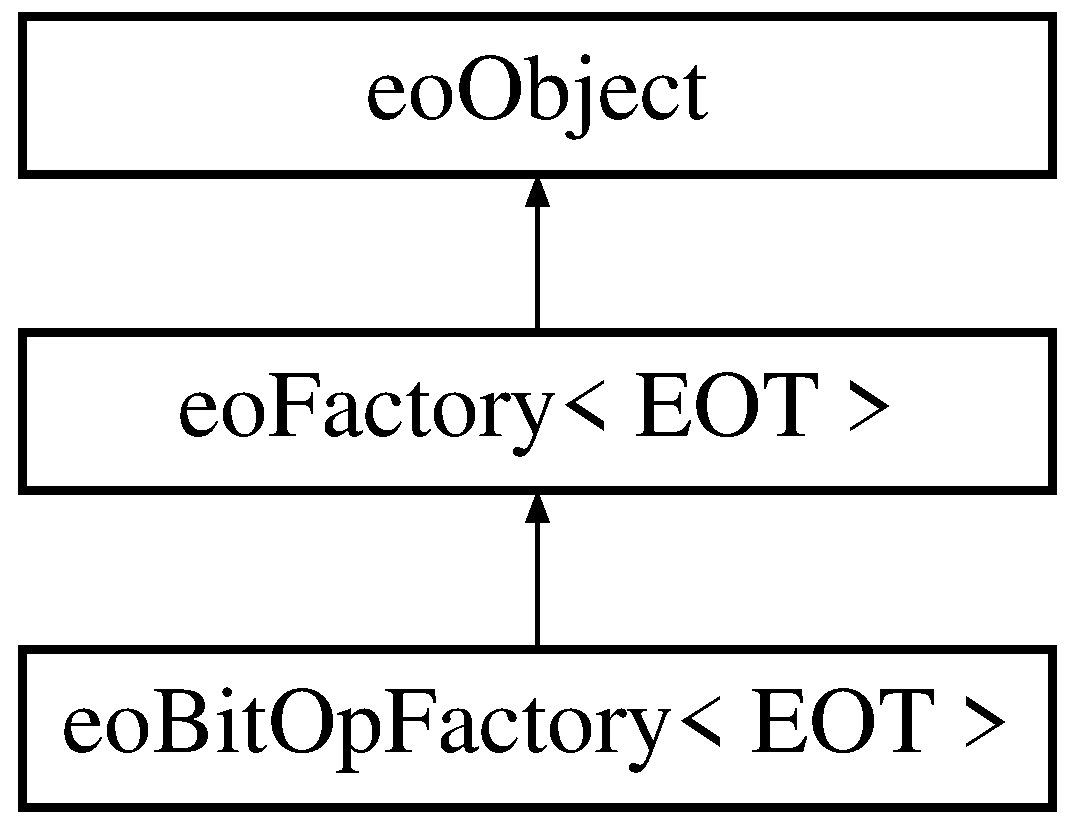
\includegraphics[height=3cm]{classeo_bit_op_factory}
\end{center}
\end{figure}
\subsection*{Public Member Functions}
\begin{CompactItemize}
\item 
virtual {\bf eo\-Op}$<$ {\bf EOT} $>$ $\ast$ {\bf make} (std::istream \&\_\-is)
\begin{CompactList}\small\item\em Another factory method: creates an object from an std::istream, reading from it whatever is needed to create the object. \item\end{CompactList}\end{CompactItemize}
\begin{Indent}{\bf ctors and dtors}\par
\begin{CompactItemize}
\item 
{\bf eo\-Bit\-Op\-Factory} ()\label{classeo_bit_op_factory_z23_0}

\begin{CompactList}\small\item\em constructor \item\end{CompactList}\item 
virtual {\bf $\sim$eo\-Bit\-Op\-Factory} ()\label{classeo_bit_op_factory_z23_1}

\begin{CompactList}\small\item\em destructor \item\end{CompactList}\end{CompactItemize}
\end{Indent}


\subsection{Detailed Description}
\subsubsection*{template$<$class EOT$>$ class eo\-Bit\-Op\-Factory$<$ EOT $>$}

{\bf EO}{\rm (p.\,\pageref{class_e_o})} Factory. 

An instance of the factory class to create operators that act on bitstring chromosomes. Only those chromosomes can instantiate the operators that are created here \begin{Desc}
\item[See also:]{\bf eo\-Select}{\rm (p.\,\pageref{classeo_select})} \end{Desc}




Definition at line 39 of file eo\-Bit\-Op\-Factory.h.

\subsection{Member Function Documentation}
\index{eoBitOpFactory@{eo\-Bit\-Op\-Factory}!make@{make}}
\index{make@{make}!eoBitOpFactory@{eo\-Bit\-Op\-Factory}}
\subsubsection{\setlength{\rightskip}{0pt plus 5cm}template$<$class EOT$>$ virtual {\bf eo\-Op}$<${\bf EOT}$>$$\ast$ {\bf eo\-Bit\-Op\-Factory}$<$ {\bf EOT} $>$::make (std::istream \& {\em \_\-is})\hspace{0.3cm}{\tt  [inline, virtual]}}\label{classeo_bit_op_factory_a0}


Another factory method: creates an object from an std::istream, reading from it whatever is needed to create the object. 

Usually, the format for the std::istream will be$\backslash$ object\-Type parameter1 parameter2 ... parametern$\backslash$ If there are problems, an std::exception is raised; it should be caught at the upper level, because it might be something for that level$\backslash$ At the same time, it catches std::exceptions thrown at a lower level, which will indicate that whatever is in the stream is for this method to process \begin{Desc}
\item[Parameters:]
\begin{description}
\item[{\em \_\-is}]an stream from where a single line will be read \end{description}
\end{Desc}
\begin{Desc}
\item[Exceptions:]
\begin{description}
\item[{\em runtime\_\-std::exception}]if the object type is not known\end{description}
\end{Desc}


Implements {\bf eo\-Factory$<$ EOT $>$} {\rm (p.\,\pageref{classeo_factory_a0})}.

Definition at line 63 of file eo\-Bit\-Op\-Factory.h.

References eo\-Factory$<$ EOClass $>$::make().

The documentation for this class was generated from the following file:\begin{CompactItemize}
\item 
eo\-Bit\-Op\-Factory.h\end{CompactItemize}
